Another important class of processes at $e^+e^-$ colliders is fermion-antifermion production, which is highly sensitive to various new physics models, as discussed in Sec.~\ref{subsec:phys_ff}. Thereby, the important observables are the polarised total cross sections, in particular in form of the left-right asymmetry \ALR, as well as the differential cross section as a function of the polar angle, $d\sigma/d \cos{\theta}$, which contains even more information than the forward-backward asymetry $A_{\mathrm{FB}}$.

\subsubsection{General experimental aspects}

At center-of-mass energies above the $Z$ pole, di-fermion production will be accompanied frequently by a significant amounts of ISR. E.g.\ at $\sqrt{s}=$250\,GeV, about half of the di-fermion events return to the $Z$ pole. The ISR photons either escape undetected through the beam pipe, or they can be produced under a sufficiently large angle to be measured in the detector {\color{red} [insert ref to detector section for calorimeter acceptance]}.

In the latter case, energy and momentum constraints can be employed to reconstruct the full event kinematics from the angles of the fermions and the photon, {\em without relying on their measured energies or momenta}. This technique offers an excellent opportunity to cross calibrate the energy scales of various subsystems, e.g.\ to calibrate the photon energy scale against the momentum scale of the tracking systems in $e^+e^- \to \mu^+\mu^-\gamma $ events. While in principle also the beam energy spectrum can be obtained from this method, it suffers from large event-by-event statistical fluctuations due to the relatively large width of the $Z$ resonance~\cite{Wilson:2016hne}.

But also in the case that there is no photon detected, the amount of collinear beamstrahlung or ISR energy can be reconstructed from kinematic constraints on an event-by-event basis. In this case, however, the measured momenta of the fermions have to be used. The previously mentioned case of $e^+e^- \to \mu^+\mu^-\gamma $, then provides an excellent method for an in-situ determination of the beam energy spectrum, since the muon momentum scale can be calibrated to 10\,ppm from $J/\psi \to \mu^+\mu^-$ decays~\cite{Wilson:2016hne}.

In presence of beam polarisation, another important observable becomes accessible, namely the left-right asymmetry of 2-fermion processes:
\begin{equation}
\ALR = \frac{\sigmaLR-\sigmaRL}{\sigmaLR+\sigmaRL}
\label{eq:defALR}
\end{equation}
Therby, \sigmaLR etc.\ are the chiral cross sections for fully polarised beams, where the first index gives the chirality of the electron and the second index the chirality of the positron. Their to the cross section for partial polarisation and the role of beam polarisation in general will be discussed in Sec.~\ref{subsec:polarization}. In this section, we will focus on the measurement of
the polarised cross sections and of angular distributions for the various 2-fermion processes.


\subsubsection{Inclusive $e^+e^- \to f\bar{f}$ analyses}
Di-fermion production at a center-of-mass energy of 250\,GeV has recently been studied both by ILD and SiD, albeit with complementary goals. ILD has performed a study of all di-lepton channels in full detector simulation, including all leptonic 2-fermion and 4-fermion backgrounds and focussing on events with $\sqrt{s'}>230$\,GeV~\cite{bib:deguchi_lcws18, Yamashiro:2018ant}. After a simple cut-based event selection, purities of 97-99\% can be obtained, while retaining a signal of 26 million events in the $e^+e^-$ case and of about 0.75 million events in the $\mu^+\mu^-$ case and 0.6 million events in the $\tau^+\tau^-$ case. The polar angle distributions of the selected events are then compared to the predictions of various BSM models, which fall into two classes: tree-level exchange of additional, $E6$-insprired $Z'$ bosons and loop-effects from dark matter candidates on the $\gamma/Z$ propagator. In the case of the $Z'$ models, the reach for a 3$\sigma$ observation ranges between 1.6 and 4.8\,TeV, depending on the exact model, while it is between 165 and 460\,GeV in case of the dark matter models, again depending on the exact type of model. These numbers so far combine only the electron and muon channels, therefore further improvement is expected once the $\tau$-channel has been included in the combination.

SiD on the other hand has performed a study focussing on the measurement of \ALR\ from radiative returns to the $Z$ pole. They studied inclusively all di-lepton and di-jet channels in fast detector simulation~\cite{bib:ueno_lcws18}. Thereby they make use of the method mentioned above in order to obtain the boost between the $Z$ rest frame and the lab frame from the angles of the two leptons or jets. After a simple cut-based event selection, about 4.5 million hadronic $Z$ events and about 0.5 million leptonic $Z$ events remain over a background of 1.2 million events for 250\,\ifb\ with \Pmp=(-80\%,+30\%). Exploiting the modified Blondel scheme~\cite{Blondel:1987wr, Monig:2001db} in order to extract \ALR\ directly from the polarised cross sections measured in the four different beam helicity configuraions, the estimated uncertainty on \ALR\ for the full 2\,\iab\ is $\Delta \ALR = 0.00039$. This number is strictly speaking a statistical uncertainty only. However, due to the redundancy offered by the presence of positron polarisation in combination with the ``quasi-concurrent'' collection of the four data sets with different beam helicity configurations, the impact of systematic uncertainties is expected to be very small, especially if \ALR\ is extracted from a global fit to several physics processes, which is, in contrast to the modified Bondel scheme, fully robust against unequal absolute polarisation values when flipping the sign of the polarisation.
For more details on the discussion of the impact of polarisation on the control of systematic uncertainties see Sec.~\ref{subsec:polarization}.

\subsubsection{$e^+e^- \to \tau^+\tau^-$}
\begin{itemize}
\item $\tau^+\tau^-$  Taikan LoI~\cite{Suehara:2009nj} and Hieu thesis?
\item decay mode separation and tau polarisation
\end{itemize}

\subsubsection{$e^+e^- \to b\bar{b}$}
\begin{itemize}
\item special difficulty: $b$ vs $\bar{b}$ jet identification (jet/vertex charge, Kaon charge, $dE/dx$ plot, role of VTX and TPC)
\item Sviatoslav's results
\end{itemize}

ILD has studied the channel $e^+e^- \to b\bar{b}$ in full, geant4-based detector simulation based on the DBD

\begin{figure*}[hbt]
       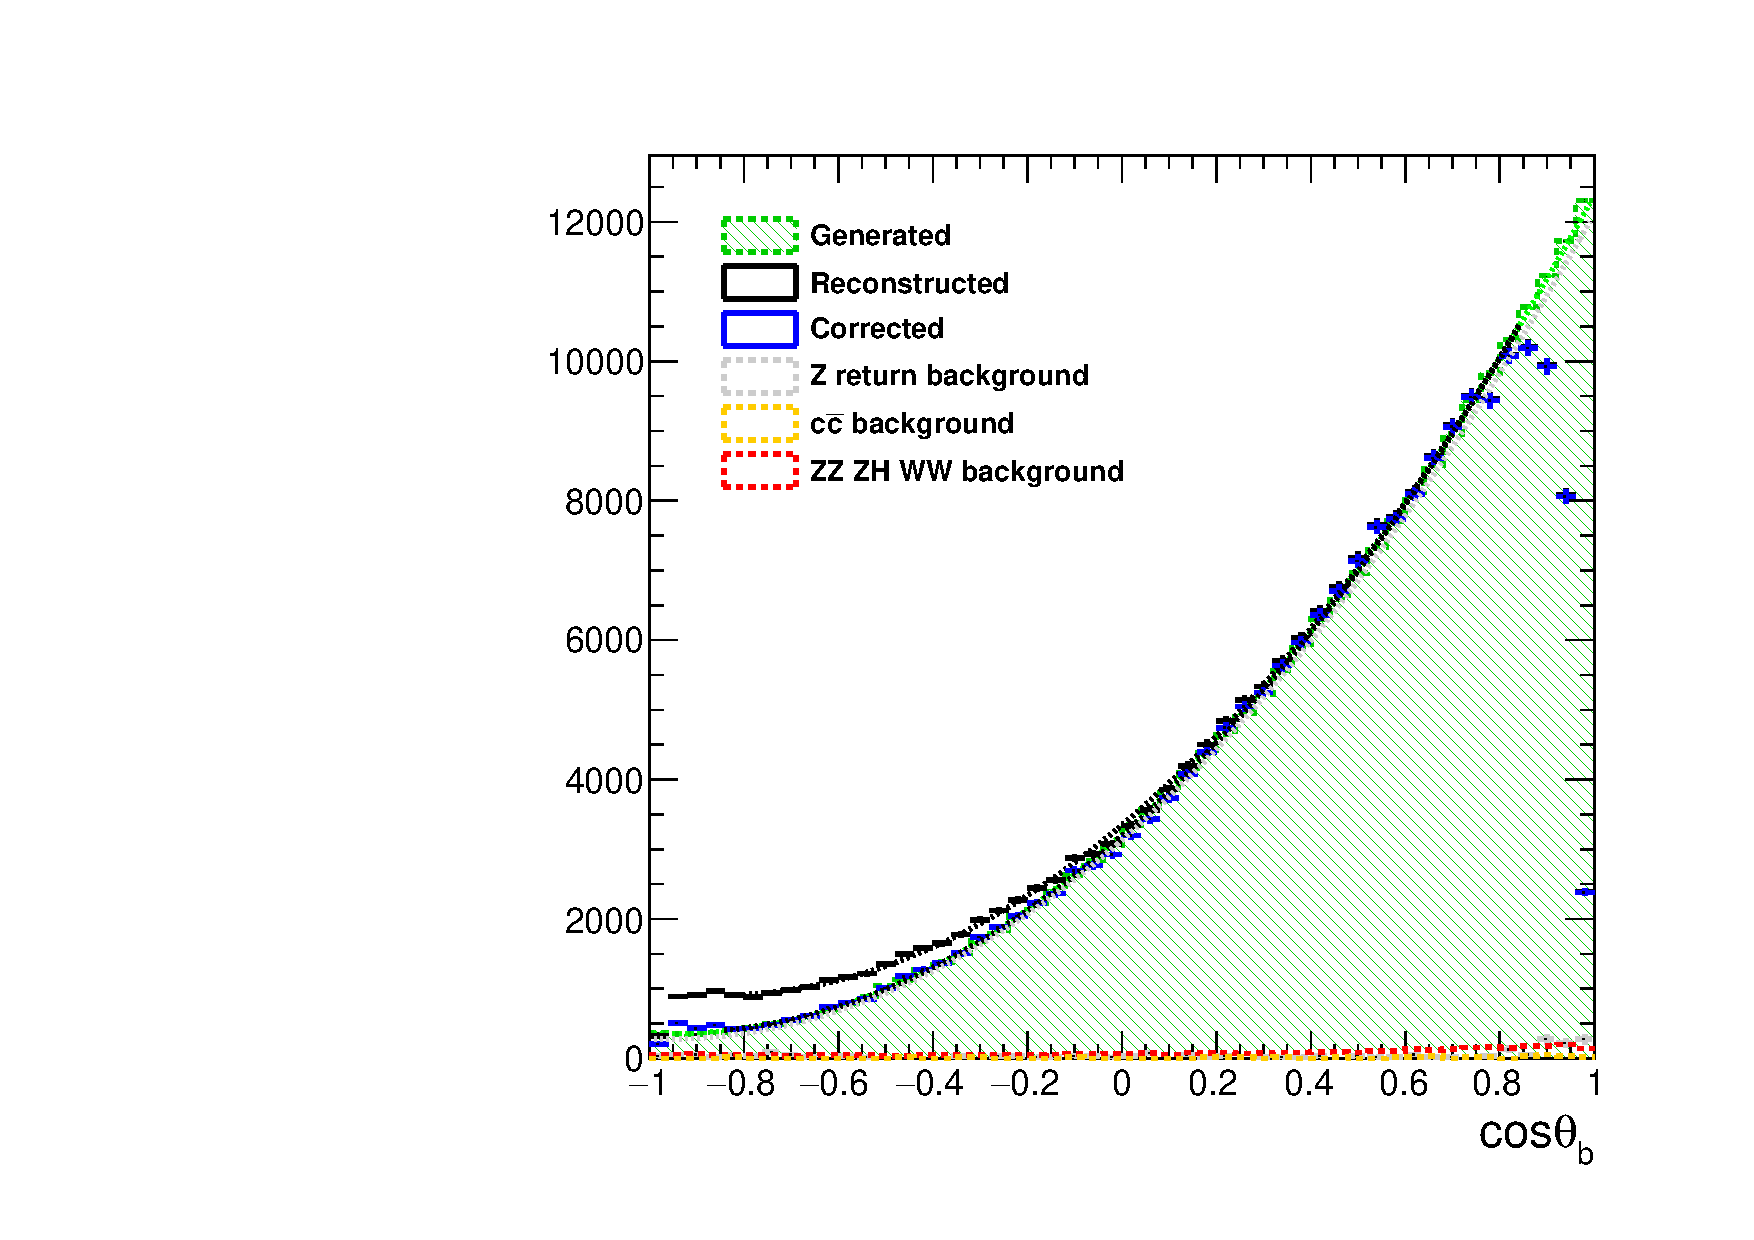
\includegraphics[width=0.4\linewidth]{./chapters/figures/basymmetry-final-left.pdf}
       \llap{\shortstack{%
                       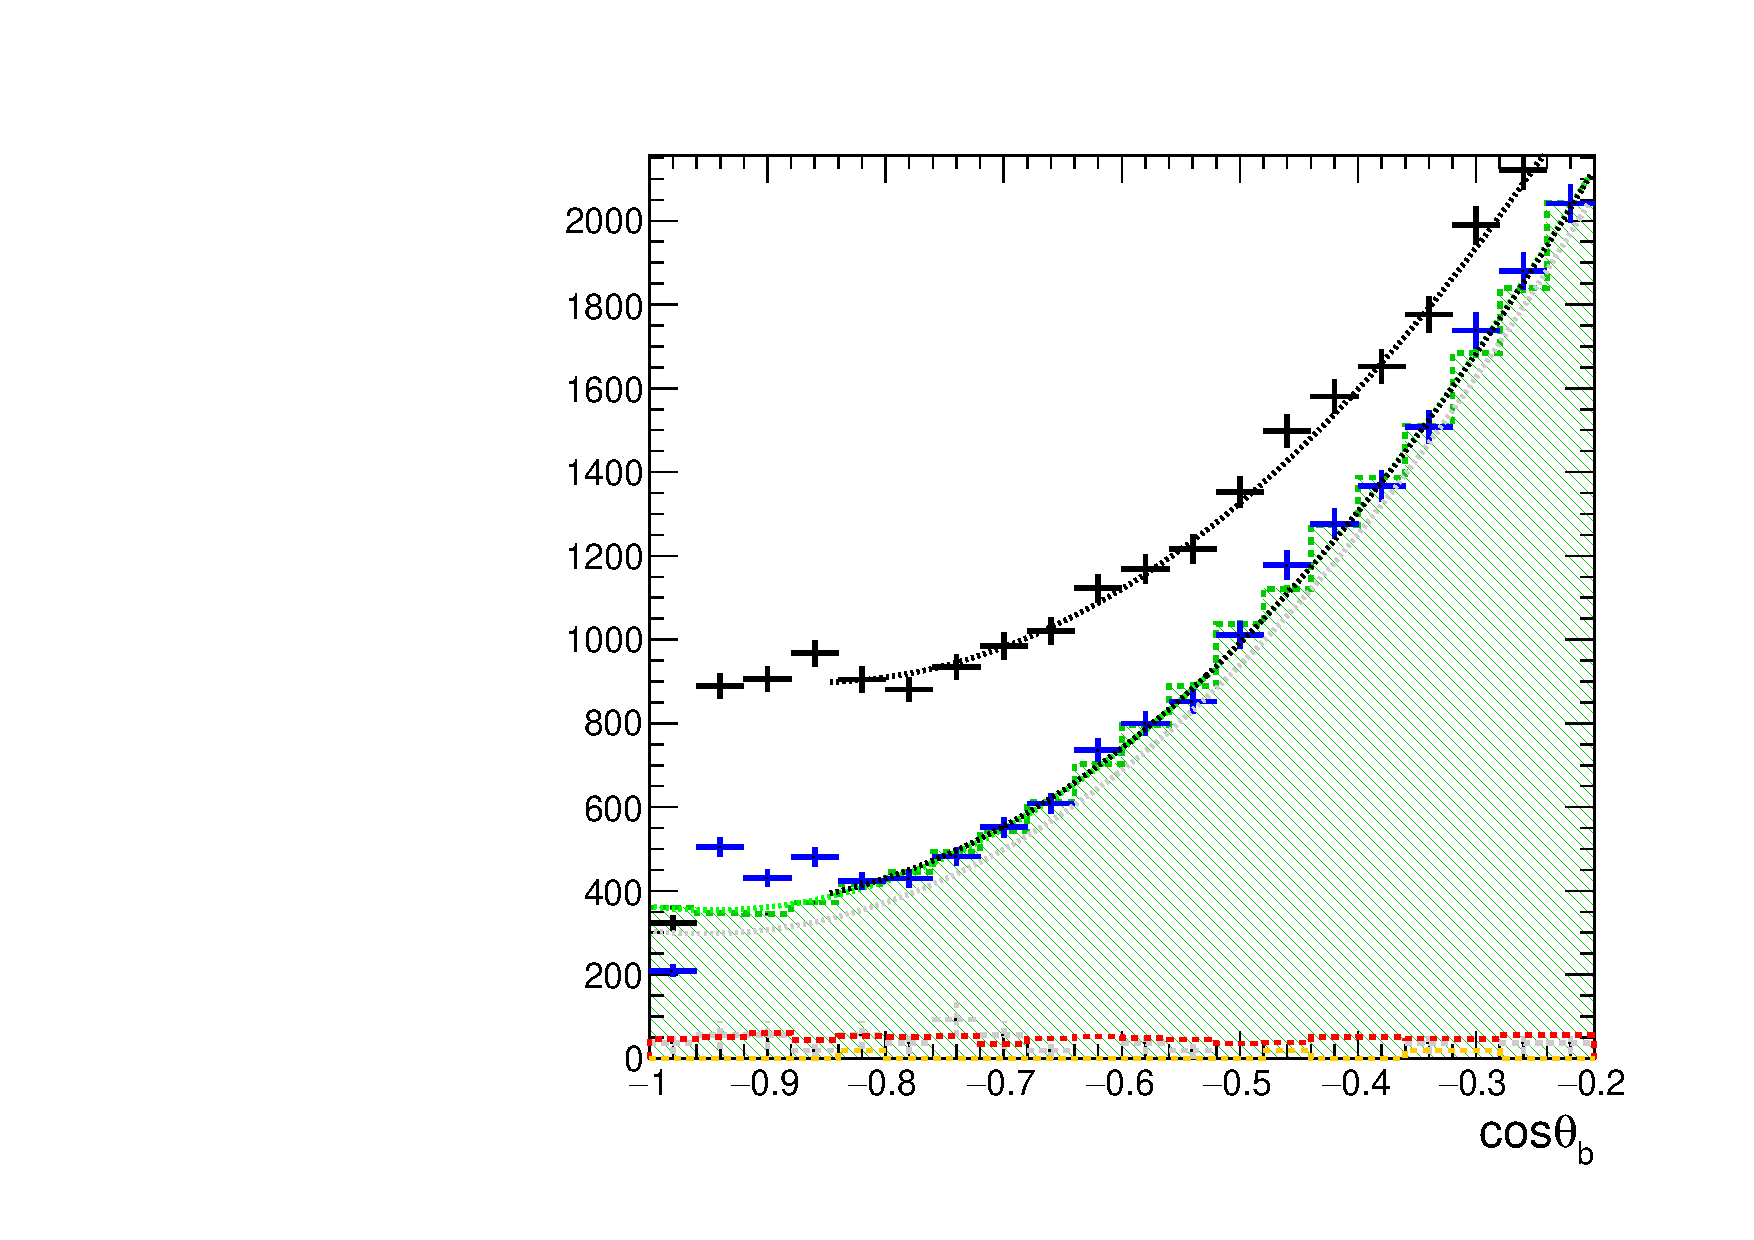
\includegraphics[clip, trim=0cm 0cm 1.8cm 1.7cm, scale=.15]{./chapters/figures/zoom-final.pdf}\\
                       \rule{0ex}{0.67in}%
               }
               \rule{2.2in}{0ex}}
        \hspace{0.2cm}       
        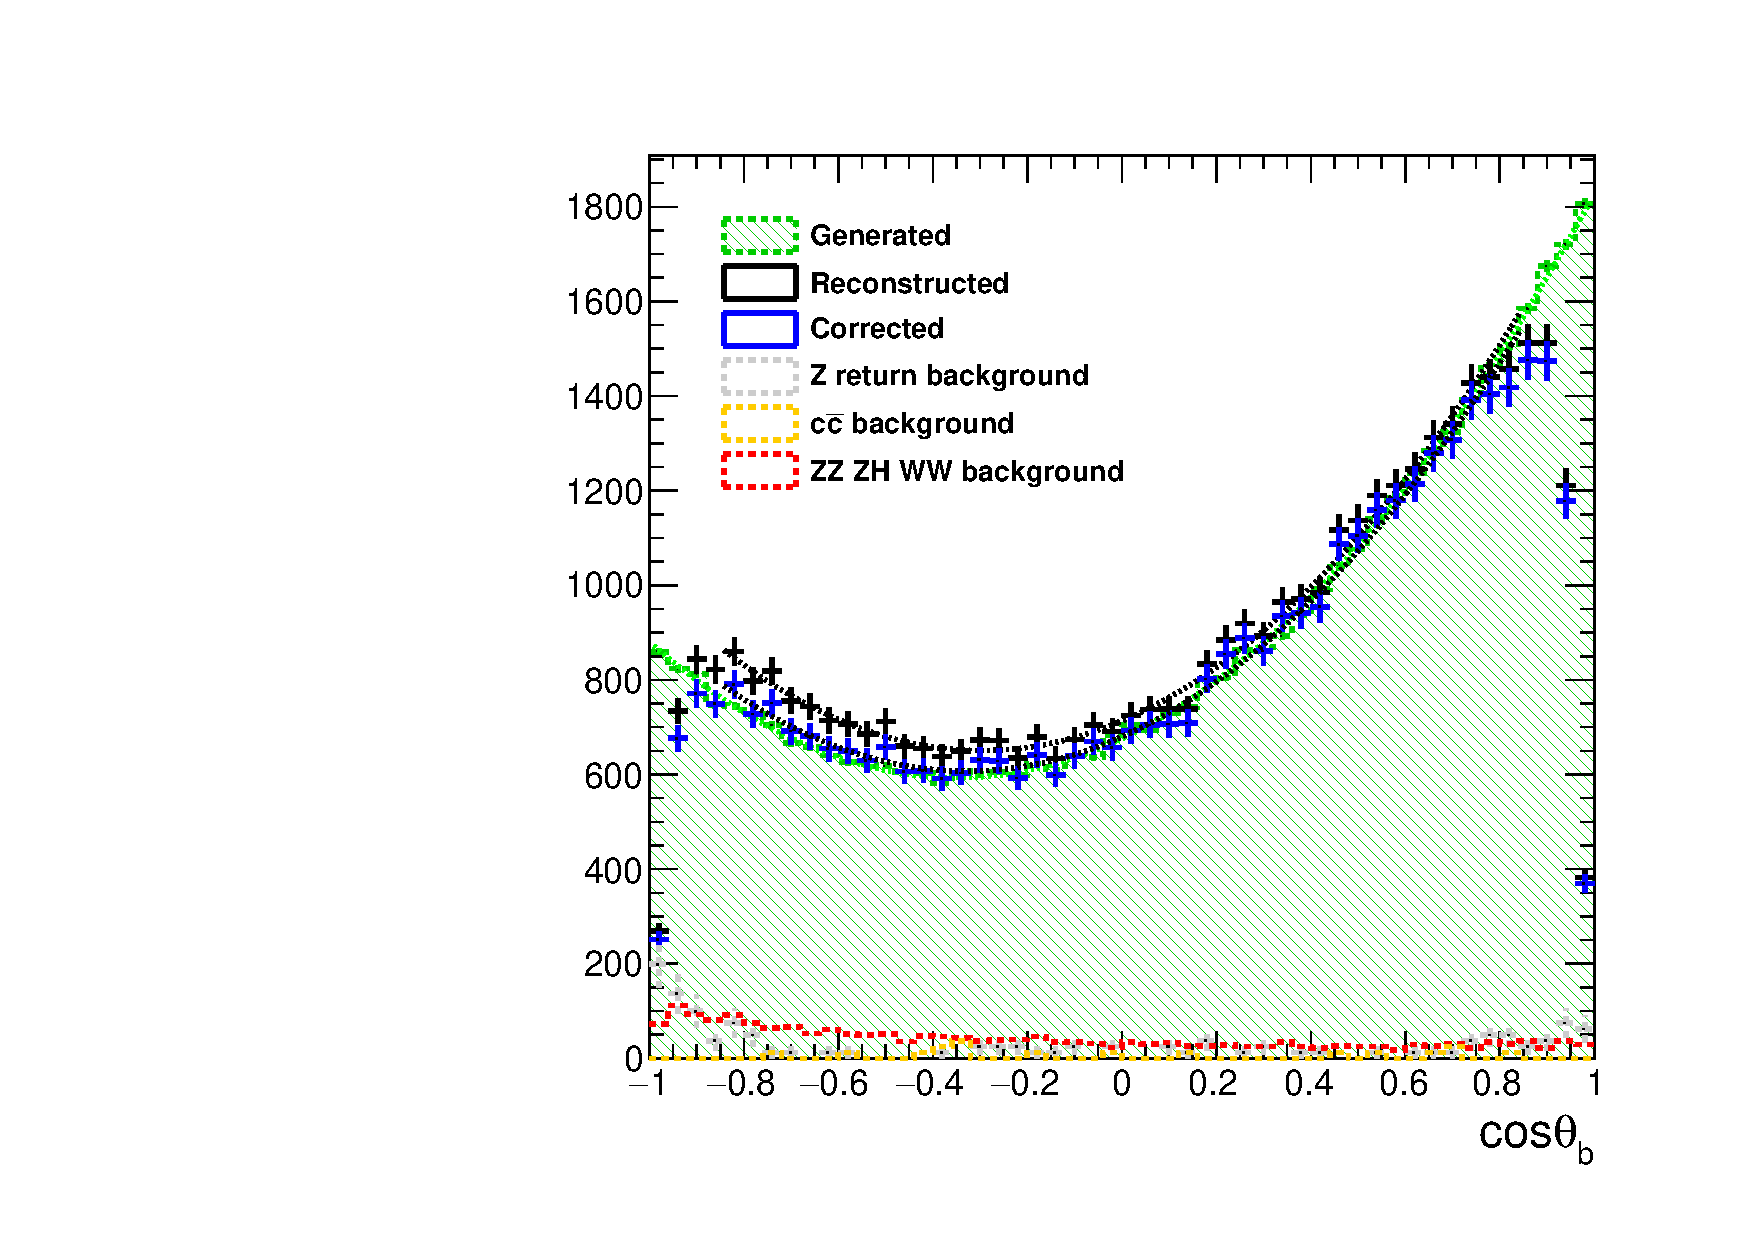
\includegraphics[width=0.4\linewidth]{./chapters/figures/basymmetry-final-right.pdf}
	\caption{Polar angle distribution $\cos{\theta_b}$ of generated $b$-quarks and final reconstructed 
         $b$-jets including any SM  background remaining after event selection. 
         Left:  $P(e^+,e^-)=(+100\%,-100\%)$ with a zoom of the region with negative 
         $\cos{\theta_b}$.
         Right: $P(e^+,e^-)=(-100\%,+100\%)$. From~\cite{Bilokin:2017lco}.  }
	\label{fig:ffbar_basym}
\end{figure*}


\begin{figure}
	\centering
	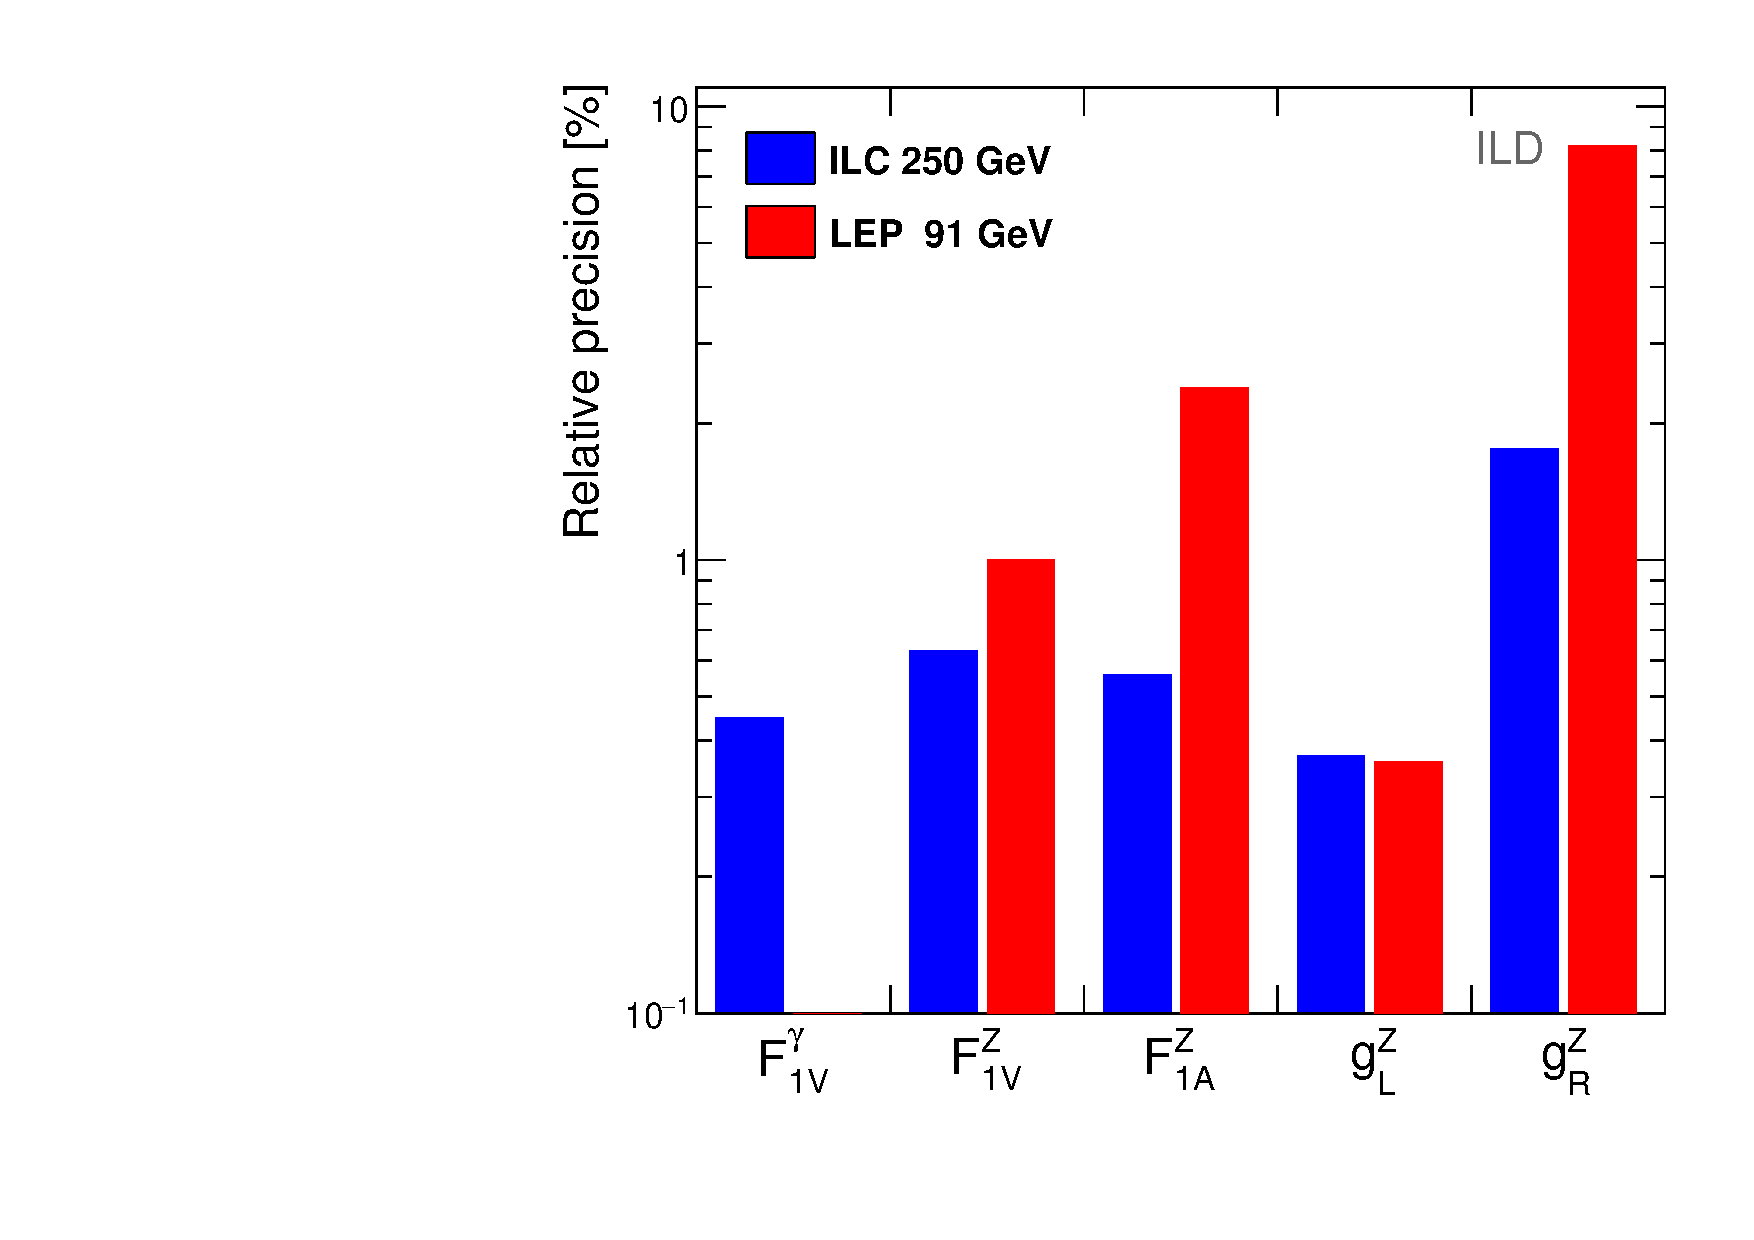
\includegraphics[width=0.8\columnwidth]{./chapters/figures/final-graph-ild.pdf}
	%	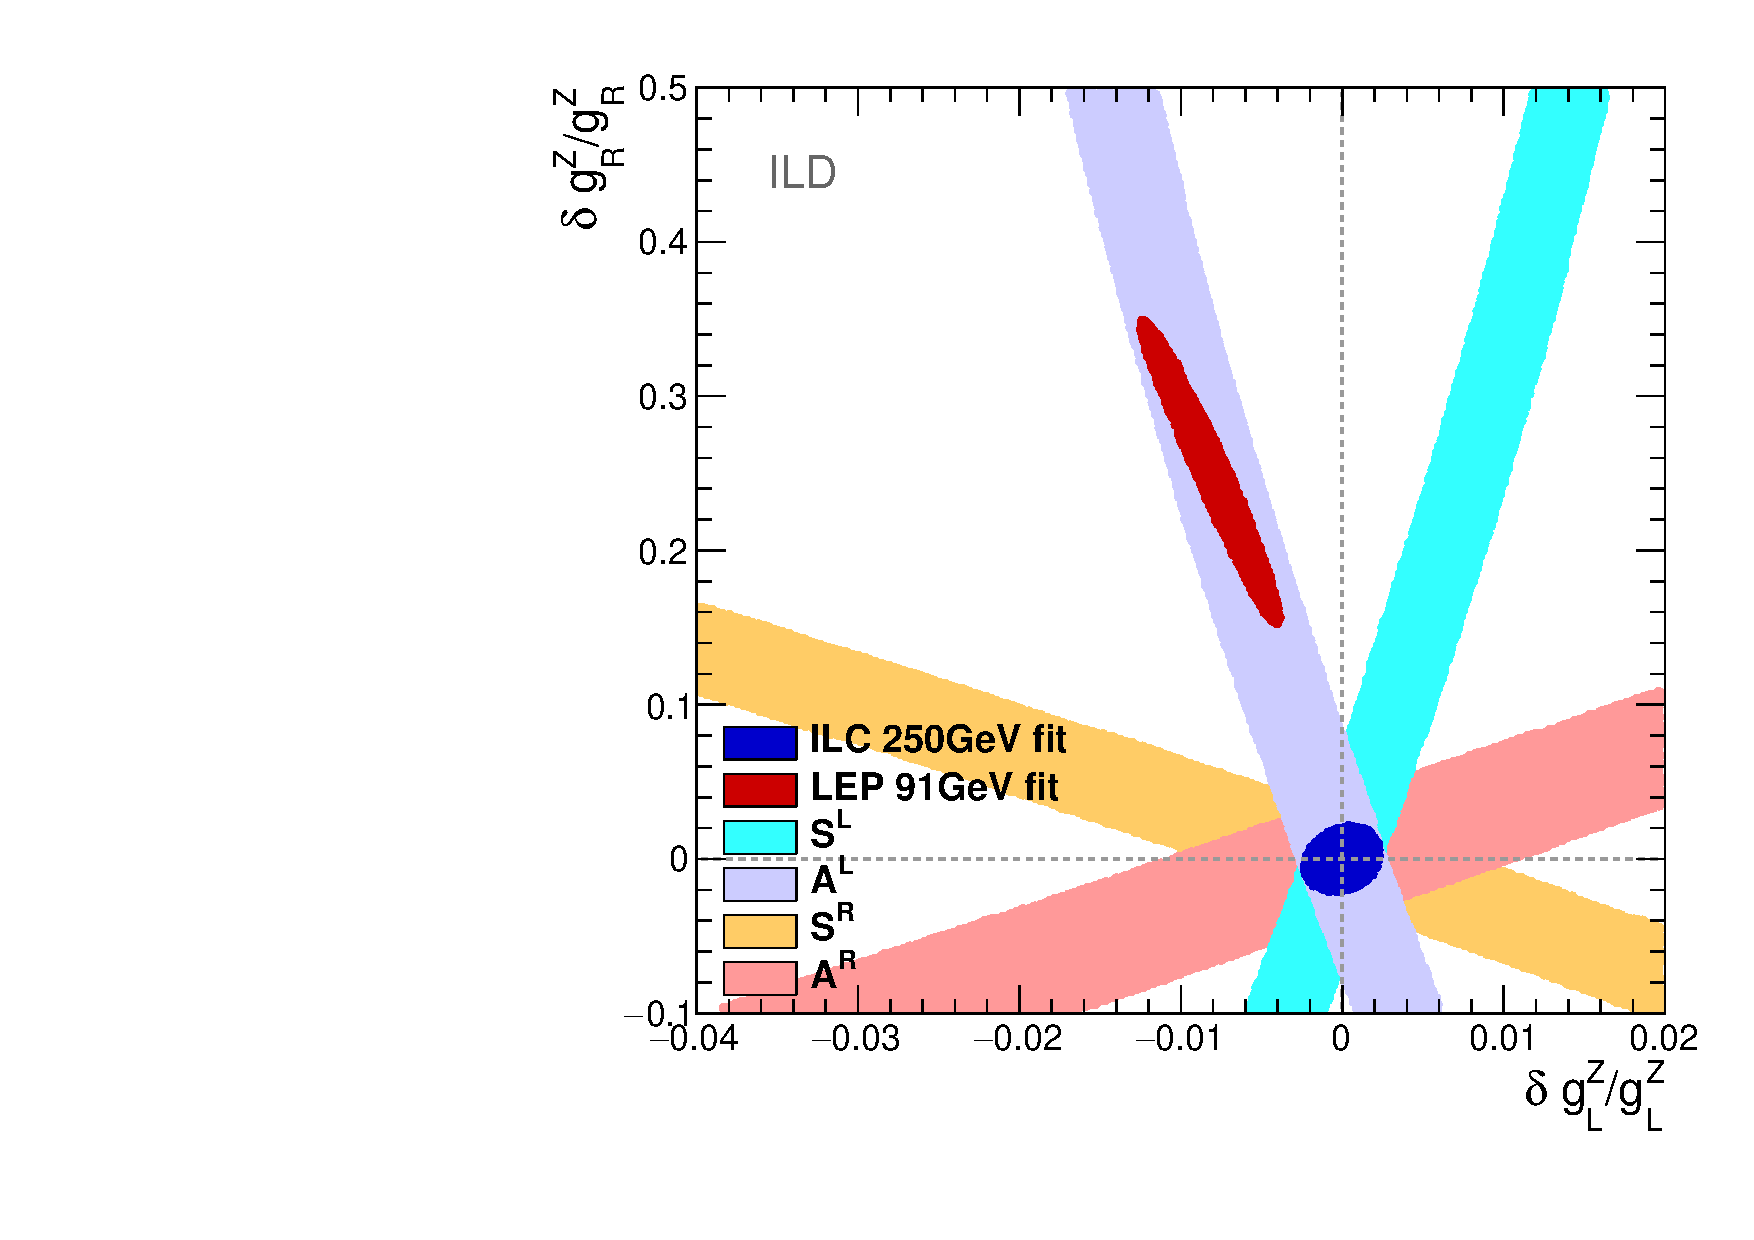
\includegraphics[width=0.95\linewidth]{./chapters/figures/ilc-precision-ild.png}
	\caption{\sl  Comparison of the LEP measurements to the expected 
                  precision at the ILC. The results of the ILC correspond to the 
                  integrated luminosity of $\mathcal{L}_I = 500$\,fb$^{-1}$ to be collected 
                   at $\sqrt{s} = 250$\,GeV before the luminosity upgrade. Final results for the
                  full 250\,GeV dataset would improve the precision further by about a factor of 2.
                   From~\cite{Bilokin:2017lco}.}
	\label{fig:LEPILCResult_3}
\end{figure}
